%%%%%%%%%%%%%%%%%%%%%%%%%%%%%%%%%%%%%%%%%%%%%%%%%%%
% introducao
\section{Motivation}

\begin{frame}{Motivation}
  \begin{itemize}
    \item Geostatistical simulations provide the means to assess the uncertainty in geological attribute models including grades and geobodies geometry.
    \item A set of realizations is generated attempting to map the uncertainty space.
    \item Simulation is an expensive computational task.
    \item There are two main methodologies to generate the realizations: Sequential Simulation and Spectral Simulation.
     \item The sequential simulation algorithm is the most used in the geostatistical framework.
  \end{itemize}
\vskip 1cm
\end{frame}

\subsection{Problem 1: How to reduce the execution time of Geostatistical Simulations?}
\begin{frame}{Problem 1}	
How to reduce the execution time of Geostatistical Simulations? 
\end{frame}

\begin{frame}{How to reduce the execution time of Geostatistical Simulations?}
	\begin{itemize}
      \item The execution time of an algorithm can be reduced using two main strategies: parallelization of the fundamental logic blocks and/or changing the key ideas used to implement the algorithm.
		\item In computer science, High Performance Computing (HPC) is a set of  Hardware and Software methodologies to reduce the execution time of complex computational tasks.    
    \end{itemize}
\end{frame}

\begin{frame}{How to reduce the execution time of Geostatistical Simulations?}
	\begin{itemize}
    	\item Algorithm parallelization is not a general solution as it is required  to identify which tasks can be executed simultaneously.
        \item Task interdependence is the main problem faced during the algorithm parallelization.
        \item  The synchronization of tasks being executed in parallel reduces the parallelization efficiency.
    \end{itemize}
\end{frame}

\begin{frame}{How to reduce the execution time of Geostatistical Simulations?}
	\begin{itemize}
    	\item Let us discuss the Problem 1.
        \item What is the best strategy to reduce the execution time of Geostatistical Simulations:
        \begin{itemize}
        	\item Parallelize the Sequential Simulation;
        	\item Use other algorithm;
        	\item Or, parallelize other algorithm?
        \end{itemize}
    \end{itemize}
\end{frame}

\subsection{Why parallelize the sequential simulation is not the best solution?}
\begin{frame}{Why parallelize the sequential simulation is not the best solution?}
	\begin{itemize}
    	\item Sequential Simulation depends on a random path  \cite{goovaerts1997geostatistics}.
        \item The random path is used to define the simulation order of the nodes.
        \item When a node is simulated, it is transformed in conditioning data.
        \item That is the problem: sometimes two or more close nodes to be simulated share the neighborhood. In other words, these two or more nodes share some conditioning data. This is called a \textbf{Conflict Zone} (Fig. \ref{conflict_zone}).
    \end{itemize}
\end{frame}

\begin{frame}{Why parallelize the sequential simulation is not the best solution?}
Conflict zone between two neighborhoods. The red stars are two points to be simulated in a given moment.
\begin{figure}[h]
  %\caption{Conflict zone between two neighborhoods. The red stars are two points to be simulated in a given moment.}
  \centering
    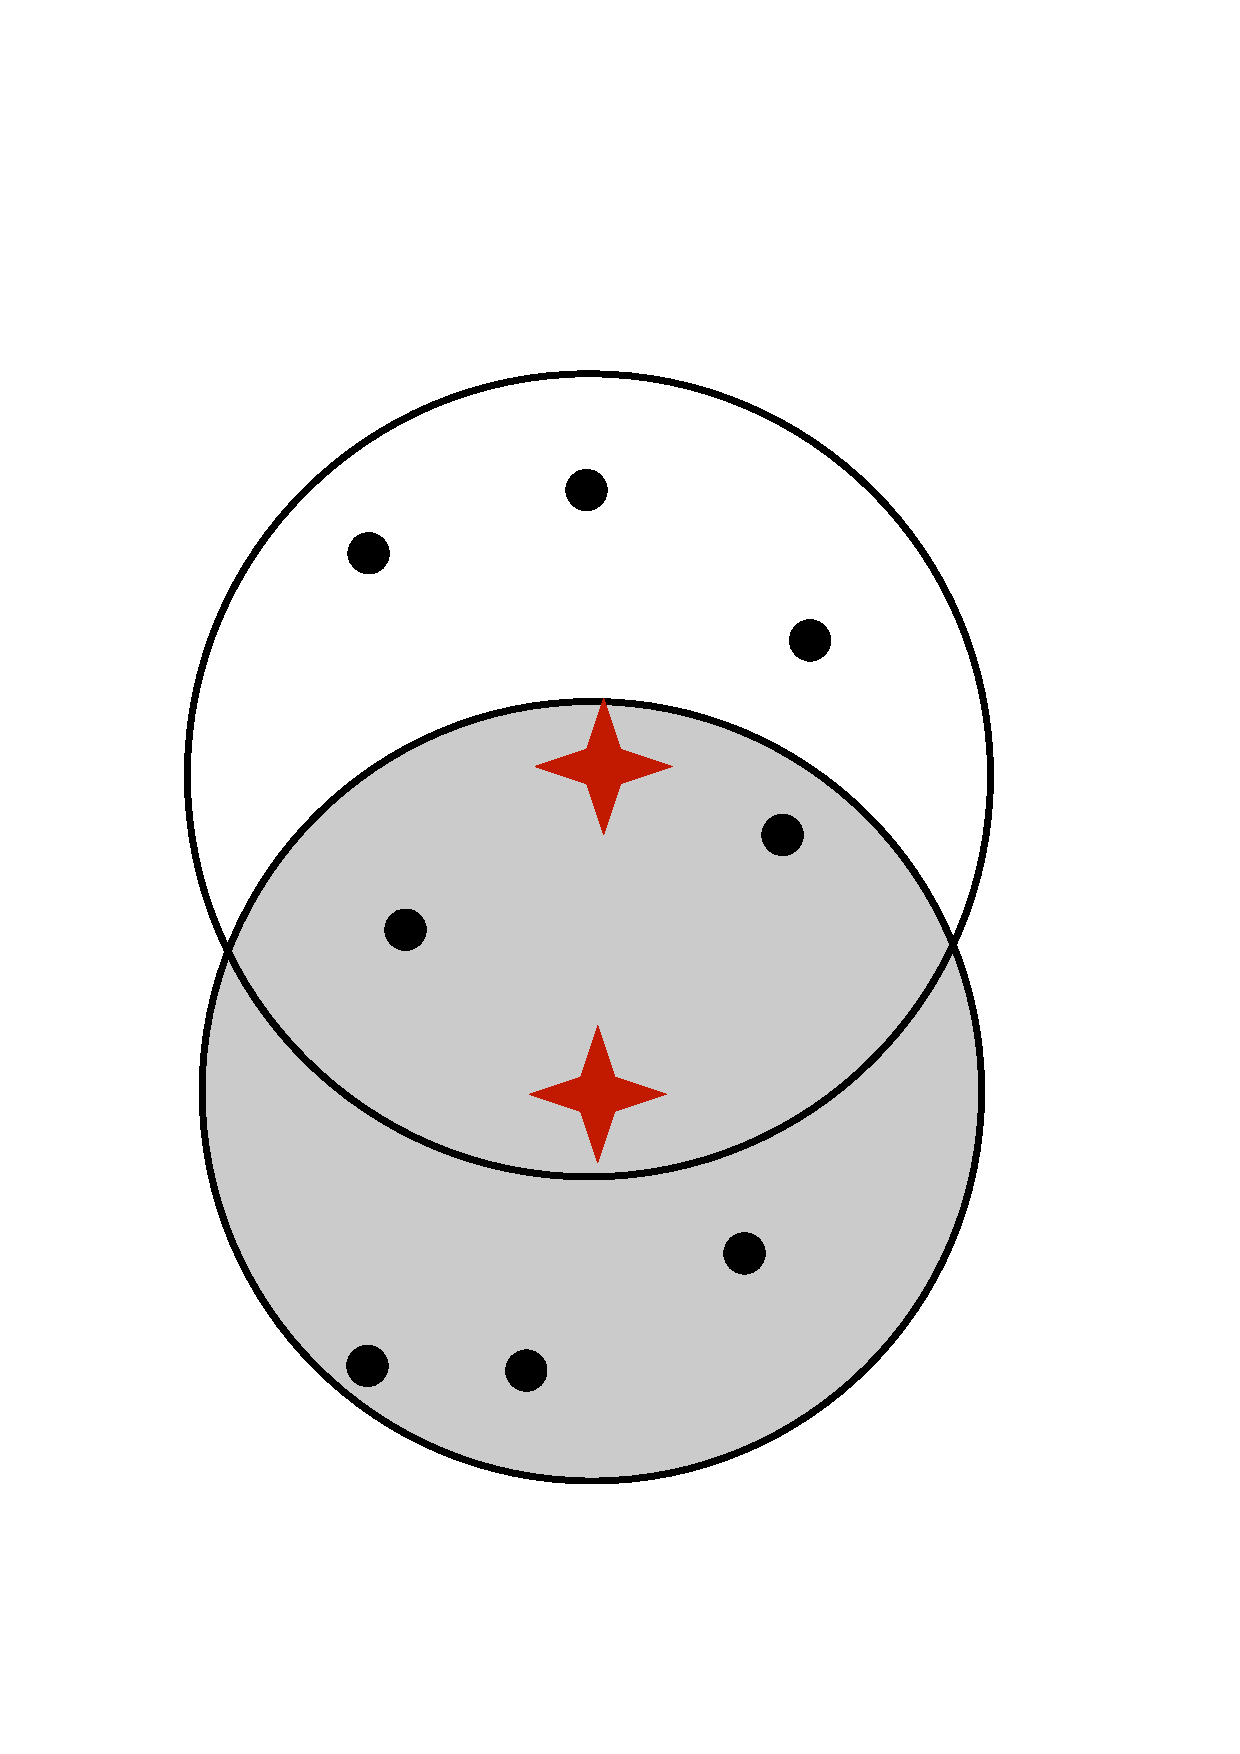
\includegraphics[width=0.4\textwidth,angle=90]{figs/conflict_zone.pdf}
    \label{conflict_zone}
\end{figure}

\end{frame}

\begin{frame}{Why parallelize the sequential simulation is not the best solution?}
	\begin{itemize}
    	\item In literature, there are five ways to deal with the conflict zones:
        \begin{enumerate}
        	\item Parallelize kriging executed during each node simulation. \cite{nunes2010parallelization}
            \item Analyze the random path to identify the nodes in non-conflicting neighborhoods and simulate them in parallel. \cite{vargas2007parallelization}
            \item Use message passage to synchronize the execution and check if a subset of nodes in the random path can be simulated in parallel. \cite{mariethoz2010general}
            \item Divide the grid in independent fields and generate the random paths for each independent field. This strategy is highly dependent on the spatial continuity model. \cite{rasera2015conflict}
            \item The trivial solution: execute in parallel the simulation of several realizations (each realization is executed using the original sequential algorithm).
        \end{enumerate}
    \end{itemize}
\end{frame}

\begin{frame}{Why parallelize the sequential simulation is not the best solution?}
	\begin{itemize}
    	\item The trivial solution is memory costly and useless during the calibration of the model parameters. Also, running in parallel several simulations of large grids demands a lot of memory, which reduces significantly the parallelization performance.
        \item Divide the grid in independent fields is a good solution when the data has a short range spatial continuity on one (some) direction. But, this is  limitation to the number of independent fields that can be simulated in parallel because the size of fields is tied to the spatial model range.
        \item Synchronize the execution steps demands the creation of a non-trivial execution manager to define the nodes or the kriging systems to be used in a given moment.
    \end{itemize}
\end{frame}


\begin{frame}{Why parallelize the sequential simulation is not the best solution?}
	\begin{itemize}
    	\item The synchronization of execution steps and the strategy to divide the grid in independent fields allow the parallelization at path level. This is useful during the parameters calibration.
        \item These are the main approaches to parallelize the Sequential Simulation. With exception of the trivial solution all solutions generate more complex version of the simulation algorithm and have limitations due the nature of the random path or the spatial continuity model. These limitations impact directly on the efficiency of the parallelization.
    \end{itemize}
\end{frame}

\subsection{Problem 2: If parallel sequential simulation is not the best approach, what would be?}
\begin{frame}{Problem 2}	
If parallel sequential simulation is not the best approach, what would be?
\end{frame}

\begin{frame}{If parallel sequential simulation is not the best approach, what would be?}
	\begin {itemize}
		\item Kriging parallelization is trivial, because to estimate each grid node is only necessary the conditioning data. Also, the conditioning data is immutable during the estimation. This allows the parallel execution of each node estimation. In computer science this type of algorithms is called \textit{embarrassingly parallel} \cite{wilkinson1999parallel}.
    
    	\item This raises a question: ``Is there some way to develop a \textit{embarrassingly parallel} simulation algorithm ?''
    \end {itemize}
\end{frame}

\begin{frame}{If parallel sequential simulation is not the best approach, what would be?}
	\begin {itemize}
		\item An \textit{embarrassingly parallel} algorithm allows the developer to use all possible parallelization strategies and technologies. And, in theory, the parallelization in this case is ``perfect'', allowing to achieve the maximum speed-up at all problem instances. 
        \item Due to random paths,  Sequential Simulation   can only be \textit{embarrassingly parallel} at a realization level, which is a big limitation when dealing with large grids.
        \item High memory usage reduces significantly the execution performance because the CPU cache is overloaded. Good use of CPU cache is one of the ways to achieve high performance.
    \end {itemize}
\end{frame}


\begin{frame}{If parallel sequential simulation is not the best approach, what would be?}
	\begin {itemize}
        \item Another issue in parallelization is synchronization which adds a sequential step to organize the parallel execution of nodes in such a way that it is not possible to use other CPU's during this step.
    	
    \end {itemize}
\end{frame}


\begin{frame}{If parallel sequential simulation is not the best approach, what would be?}
	\begin{itemize}
    	\item So, to answer the question before mentioned: Yes, there is a way to develop an \textit{embarrassingly parallel} simulation algorithm. 
    \end{itemize}
\end{frame}


\section {Thesis statement}
\begin{frame}{Thesis statement}
The previous discussion presented the thesis motivation statement:


\begin{block}{}
``High performance computing applied to spectral simulation is a better approach to develop parallel simulation algorithms.''
\end{block}

\end{frame}
